\documentclass[12pt,twocolumn]{article}
\usepackage[margin=1.5cm]{geometry}
\usepackage{amsmath}
\usepackage{graphicx}
\usepackage{hyperref}
\usepackage{sectsty}
\title{Midterm 1}
\author{Prof. Jordan C. Hanson}
\sectionfont{\fontsize{12}{15}\selectfont}

\begin{document}
\maketitle
\small

\section{Unit 0: Electrostatics I and II}

\noindent
\begin{enumerate}
\item A 50 gram copper wire has a net charge of 2.00 $\mu$C. What fraction of the copper’s electrons has been removed? (Each atom has 29 protons, and the atomic mass is 63.5.) \\ \vspace{2cm}
\item A test charge of +2 $\mu$C is placed halfway between a charge of +6 $\mu$C and another of +4 $\mu$C separated by 10 cm. (a) What is the magnitude of the net force on the test charge? (b) What is the direction of this force (away from or toward the +6 $\mu$C charge)? \\ \vspace{3cm}
\item What is the force on the charge located at $x=8.00$ cm in Fig. \ref{fig:e-field_1}(a) given that $q=1.00$ $\mu$C?
\begin{figure}[hb]
\centering
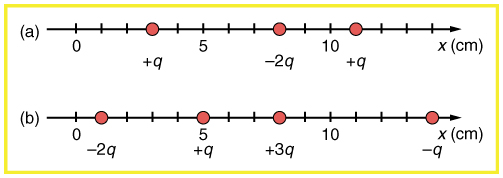
\includegraphics[width=0.49\textwidth]{e-field_1.jpeg}
\caption{\label{fig:e-field_1} Linear arrangement of charges.}
\end{figure}
\item Find the total electric field at $x=11.00$ cm in Fig. \ref{fig:e-field_1}(b). \\ \vspace{5cm}
\item Determine the direction of the force on $q$ in Fig. \ref{fig:e-field_2}, given that $q_a=q_b=+7.50$ $\mu$C and $q_c = q_d = -7.50$ $\mu$C. (b) Calculate the force on the charge $q$, given that the square is 10.0 cm on a side and $q=2.00$ $\mu$C.
\begin{figure}[hb]
\centering
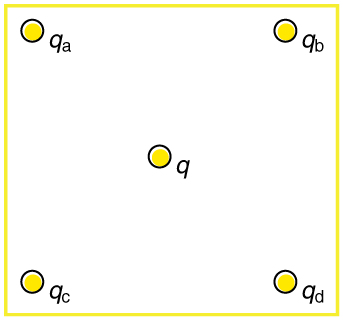
\includegraphics[width=0.25\textwidth]{e-field_2.jpeg}
\caption{\label{fig:e-field_2} 2D arrangement of charges.}
\end{figure} \vspace{3cm}
\item (a) An evacuated tube uses an accelerating voltage of 40 kV to accelerate electrons to hit a copper plate and produce x rays. Non-relativistically, what would be the maximum speed of these electrons? (b)  Show that units of V/m and N/C for electric field strength are indeed equivalent. \\ \vspace{3cm}
\item The electric field strength between two parallel conducting plates separated by 4.00 cm is $7.50 \times 10^4$ V m$^{-1}$. (a) What is $\Delta V$ between the plates? (b) The plate with the lowest potential is taken to be at zero volts. What is the potential 1.00 cm from that plate (and 3.00 cm from the other)? (c) The voltage across a membrane forming a cell wall is 80.0 mV and the membrane is 9.00 nm thick. What is the electric field strength?\footnote{The value is surprisingly large, but correct.} \\ \vspace{4cm}
\item A doubly charged ion is accelerated to an energy of 32.0 keV by the electric field between two parallel conducting plates separated by 2.00 cm. What is the electric field strength between the plates? \\ \vspace{2cm}
\item In one of the classic nuclear physics experiments at the beginning of the 20th century, an alpha particle was accelerated toward a gold nucleus, and its path was substantially deflected by the Coulomb interaction. If the energy of the doubly charged alpha nucleus was 5.00 MeV, how close to the gold nucleus (79 protons) could it come before being deflected? \\ \vspace{3cm}
\end{enumerate}

\section{Unit 1: Capacitors, Current, and DC \\ circuits}

\noindent
\begin{enumerate}
\item What capacitance is needed to store 3.00 $\mu$C of charge at a voltage of 120 V? \\ \\
\item (a) What is the energy stored in the 10.0 $\mu$F capacitor of a heart defibrillator charged to $9.00\times 10^3$ V? (b) Find the amount of stored charge. (c) In open heart surgery, a much smaller amount of energy will defibrillate the heart.  What voltage is applied to the 8.00 $\mu$F capacitor of a heart defibrillator that stores 40.0 J of energy? (d) Find the amount of stored charge. \\ \vspace{4cm}
\item To build up the charge and energy required in part (a) of the previous problem, an AED designer decides to split the charge among four capacitors in parallel.  Determine the required capacitance of each individual capacitor, and the charge stored on each, if the voltage remains $9.00 \times 10^3$ V.  Why would the designer choose not to connect the capacitors in series? \\ \vspace{5cm}
\item If a 1.0 mm diameter copper wire can have a resistance of no more than 2.0 $\Omega$, (at 20 degrees C), how long can it be? \\ \vspace{3cm}
\item An LED is connected in series with a 1 k$\Omega$ resistor.  A 3.0V battery is connected to the resistor, the LED follows the resistor, and the LED is then connected to ground.  The negative terminal of the battery is also connected to ground.  (a) What current flows from the battery, if the LED resistance is $3$ $\Omega$? (b) How much power is consumed by the LED? (c) How many Coulombs of charge flow through the LED in 10 minutes? \\ \vspace{3cm}
\end{enumerate}

\section{Unit 2: DC circuits with resistors in \\ series and parallel, RC circuits}

\begin{figure}
\centering
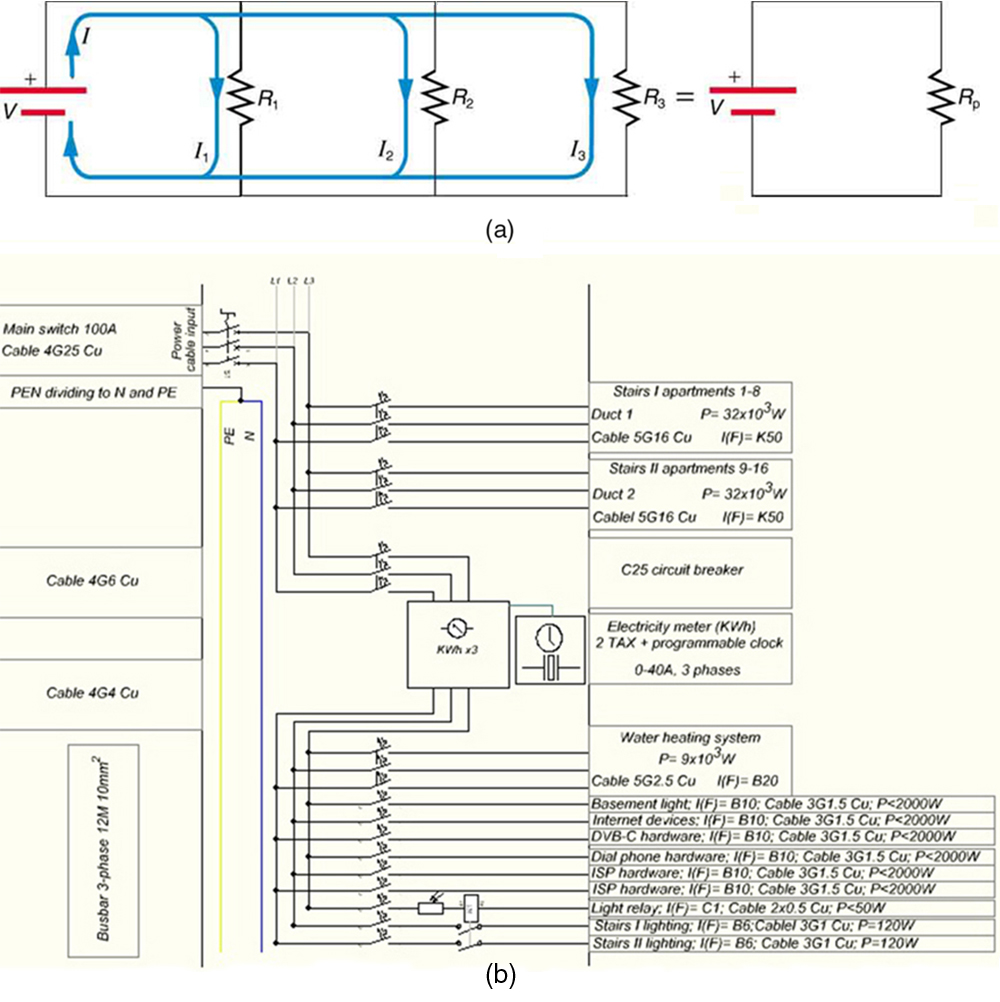
\includegraphics[width=0.4\textwidth,trim=0cm 13.5cm 5.5cm 0cm,clip=true]{parallel.jpeg}
\caption{\label{fig:para} \small A DC circuit with three resistors.}
\end{figure}
\begin{figure}
\centering
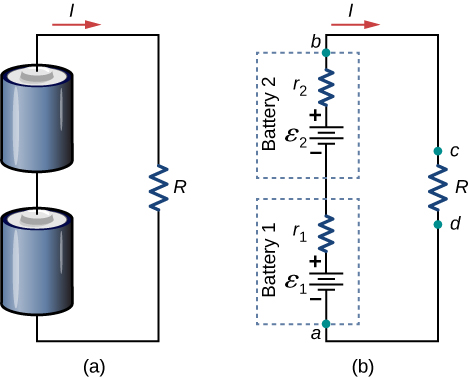
\includegraphics[width=0.13\textwidth,trim=0cm 0.5cm 4cm 0cm,clip=true]{series_batt.jpg}
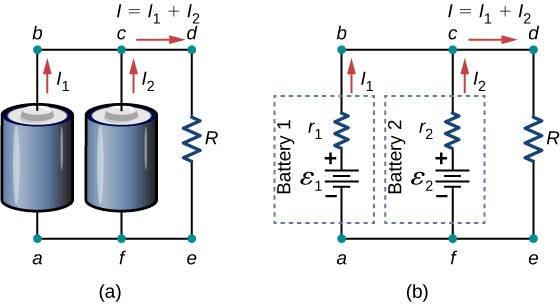
\includegraphics[width=0.18\textwidth,trim=0cm 0.5cm 5.5cm 0.41cm,clip=true]{parallel_batt.jpg}
\caption{\label{fig:batt} \small (Left) A DC circuit with two batteries in series, and a resistance $R = 0.5$ k$\Omega$. (Bottom) A DC circuit with two batteries in parallel, and a resistance $R = 0.5$ k$\Omega$.}
\end{figure}
\begin{enumerate}
\item In Fig. \ref{fig:para}, let $R_1 = 10$ k$\Omega$, $R_2 = 5$ k$\Omega$, and $R_{\rm tot} = 2$ k$\Omega$.  (a) What is the resistance of $R_3$? (b) If the battery has $\Delta V = 12$ V, what current flows from the battery? (c) What are the individual currents, $I_1$, $I_2$, and $I_3$? \\ \vspace{3.5cm}
\item Consider Fig. \ref{fig:batt}. (a) Assuming no internal resistance, calculate the current and power through the resistance $R$ if each battery has 1.5 V in the series circuit, and 3 V in the parallel circuit. (b) Now repeat part (a) for each circuit, assuming all batteries have an internal resitance of $5$ $\Omega$. \\ \vspace{3cm}
\item A child's electronic toy is supplied by three 1.58-V alkaline cells having internal resistances of 0.02 $\Omega$ in series with a 1.53-V carbon-zinc dry cell having a 0.10 $\Omega$ internal resistance. The load resistance is 10.00 $\Omega$. (a) Draw a circuit diagram of the toy and its batteries. (b) What current flows? (c) How much power is supplied to the load? (d) What is the internal resistance of the dry cell if it goes bad, resulting in only 0.500 W being supplied to the load? \\ \vspace{4cm}
\item A heart pacemaker fires 72 times a minute, each time a 25.0-nF capacitor is charged (by a battery in series with a resistor) to 0.632 of its full voltage. What is the value of the resistance? \\ \vspace{5cm}
\item An ECG monitor must have an RC time constant less than $1.00 \times 10^2$ $\mu$s to be able to measure variations in voltage over small time intervals. If the resistance of the circuit (due mostly to that of the patient’s chest) is 1.00 k$\Omega$, what is the maximum capacitance of the circuit? \\
\end{enumerate}

\section{Unit 3: Magnetism I}
\begin{figure}
\centering
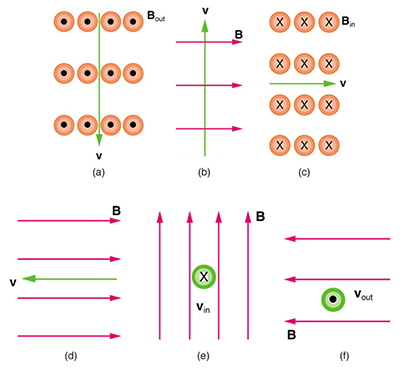
\includegraphics[width=0.4\textwidth,trim=0cm 2.8cm 0cm 0cm,clip=true]{Bfield.jpeg}
\caption{\label{fig:B} Three cases involving the particle velocity $\vec{v}$, and $\vec{B}$ field.}
\end{figure}
\begin{figure}
\centering
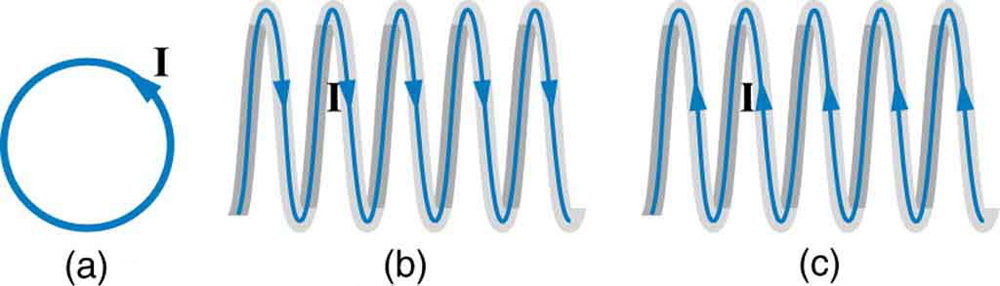
\includegraphics[width=0.4\textwidth]{coils.jpeg}
\caption{\label{fig:B2} Three currents that create B-fields.}
\end{figure}

\noindent
\begin{enumerate}
\item Consider Fig. \ref{fig:B}. Fill in Tab. \ref{tab:ex} of directions below for the Lorentz force, assuming a \textbf{negatively charged} particle.  Let $\hat{i}$ represent right, $\hat{j}$ represent up, and $\hat{k}$ represent out of the page.
\begin{table}
\centering
\begin{tabular}{| c | c | c | c |}
\hline
Case & v direction & B direction & F direction \\ \hline
(a) & & & \\ \hline
(b) & & & \\ \hline
(c) & & & \\ \hline
(d) & & & \\ \hline
\end{tabular}
\caption{\label{tab:ex} Table of directions for to Fig. \ref{fig:B}.}
\end{table}
\item An electron moving at $4.00\times 10^3$ m s$^{-1}$ in a 1.25-T magnetic field experiences a magnetic force of $1.40\times 10^{-16}$ N. What angle does the velocity of the electron make with the magnetic field? There are two possible answers. \\ \vspace{5cm}
\item (a) An oxygen-16 ion with a mass of $2.66\times 10^{-26}$ kg travels at $5.00\times 10^6$ m/s perpendicular to a 1.20-T magnetic field, which makes it move in a circular arc with a 0.231-m radius. What positive charge is on the ion? (b) What is the ratio of this charge to the charge of an electron? (c) Discuss why the ratio found in (b) should be an integer. (d) A mass spectrometer is being used to separate common oxygen-16 from the much rarer oxygen-18, taken from a sample of old glacial ice. (The relative abundance of these oxygen isotopes is related to climatic temperature at the time the ice was deposited.) The ratio of the masses of these two ions is 16 to 18.  Assuming the ions have the same charge, what would the radius of the circular arc be for the oxygen-18?  \textit{Hint: this is a scaling problem.} \\ \vspace{6cm}
\item What force is exerted on the water in an MHD drive utilizing a 25.0-cm-diameter tube, if 100-A current is passed across the tube that is perpendicular to a 2.00-T magnetic field? (The relatively small size of this force indicates the need for very large currents and magnetic fields to make practical MHD drives.) \\ \vspace{3cm}
\item For this exercise, we are designing an electric motor.  Calculate the B-field strength needed on a 200-turn square loop 20.0 cm on a side to create a maximum torque of 300 N m if the loop has 25.0 A of current.  \\ \vspace{5cm}
\item Consider Fig. \ref{fig:B2}.  Fill in the B-field directions in Tab. \ref{tab:ex2} using Amp\`{e}re's Law, and the appropriate right-hand rule. Let $\hat{i}$ represent right, $\hat{j}$ represent up, and $\hat{k}$ represent out of the page.
\begin{table}
\centering
\begin{tabular}{| c | c |}
\hline
Case & B direction \\ \hline
(a) & \\ \hline
(b) & \\ \hline
(c) & \\ \hline
\end{tabular}
\caption{\label{tab:ex2} Table of directions for to Fig. \ref{fig:B2}.}
\end{table}
\item Calculate the size of the magnetic field 20 m below a high voltage power line. The line carries 450 MW at a voltage of 300,000 V. \\ \vspace{3cm}
\item The B-field in the tokamak reactor in Fig. \ref{fig:B3} is given by $B = \mu_0 N I / (2\pi r)$, where $N$ is the total number of loops, $I$ is the current, and $r$ is the radius at which we evaluate the B-field.  (a) Design your own reactor by specifying practical values of $N$, $I$, and $r$ that achieve a 1.0 T B-field at a radius of 5.0 m.  (b) With what frequency will a proton circle the toroidal B-field (1.0 T)?  \textit{These ideas will help activate fusion reactors.}
\end{enumerate}
\begin{figure}[hb]
\centering
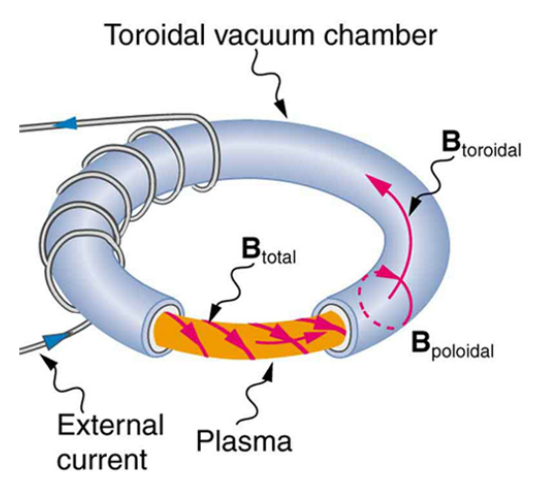
\includegraphics[width=0.33\textwidth]{tokamak.png}
\caption{\label{fig:B3} A generalized diagram of a tokamak.}
\end{figure}
\end{document}